\section{Experimental Results}


\begin{table}
\caption{Properties of the outer valence spectra of mixed ArXe clusters. Spectra of pure Ar and Xe clusters are included for reference. All spectra were recorded at $h\nu = 17$~eV, except for the pure Xe clusters ($h\nu = 60$~eV). Binding energies $E_b$ were determined as the centre of gravity of the respective feature, while band width $w$ are the FWHM of a Gaussian fit. The experimental Xe content of the clusters always is higher than in the original gas mixture (see Tab.\ \protect\ref{tab:cluster}). It was determined from the areas of the respective photolines, corrected by the respective atomic photoionization cross sections (Ar 33.0 Mb, Xe 51.3 Mb)\cite{samson2002}. Uncertainties are estimated as 3\,\% for the Xe content and 0.05~eV for the binding energies. Labels given in the first column refer to the expansion parameters in Tab.\ \protect\ref{tab:cluster}. $E_b$ and $w$ are in eV, $A$ is in \%. The binding energies can be compared to atomic values of 15.82~eV, 13.43~eV and 12.13~eV for Ar 3p and Xe 5p.
\label{tab:valence} }
\begin{tabular}{ l c c c c c c}
%
\toprule
  label & $E_b$(Ar 3p) & $w$(Ar 3p) & $E_b$(Xe 5p$_{1/2}$) &  $E_b$(Xe 5p$_{3/2}$) & $w$(Xe 5p$_{3/2}$)  &  $A$(Xe) \\
%
\midrule
% Ar, from Marko
 Ar (1) &  15.3  &  1.1 & & & &  \\
% Ar, from Marko 
 Ar (2) &  15.1  &  1.3 & & & &  \\
%
%  columns in the following: energies c.g. 51-plt-oval, widths Marko Diss., Xe content Marko Diss
% 1103 676, 679
 (a) & 15.36 & 0.9 & 13.07 & 11.75 & 0.85 & 12\\
% 1103 670
 (b) & 15.30 & 1.0 & 12.97 & 11.61 & 0.85 & 11\\
% 1103 671
 (c) & 15.25 & 1.1 & 12.91 & 11.52 & 1.08 & 10\\
% 1103 663
 (d) & 15.39 & 0.8 & 13.06 & 11.68 & 1.02 & 29\\
% 1103 640
 (e) & 15.31 & 0.6 & 12.96 & 11.44 & 1.24 & 53\\
% 0506 
Xe (1) & & & 12.76 & 11.19 & 1.18 & 100\\
%
\midrule
%
%  1004  886  (UHe, c.g. + roi values)
 886 & 15.15 & 1.3 & 12.59 & 11.01 & 1.24 & 19\\
\bottomrule
\end{tabular}
\end{table}


\begin{figure}[ht]
 \centering
 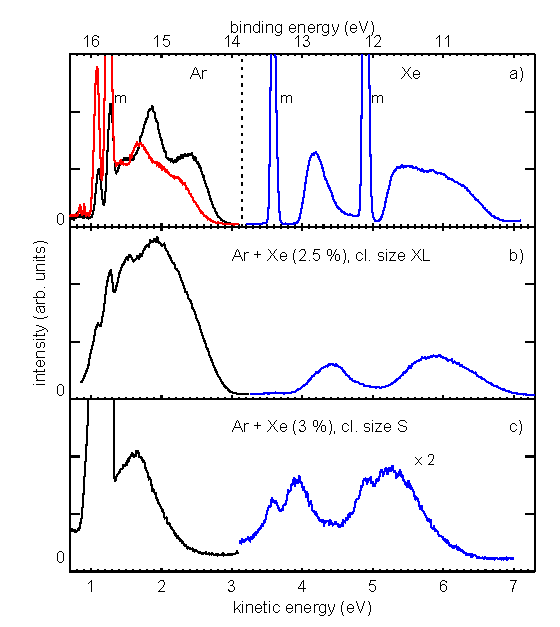
\includegraphics[width=8.5cm]{pics/figure_oval_1.pdf}
 \caption{
 Outer valence spectra of mixed Ar-Xe clusters, in comparison to the pure species. Panel a) shows the outer valence region of homogeneous Ar and Xe clusters, respectively (see text for details). The two lower panels show the spectra of the mixed species of different size. Sharp lines marked `m' result from photoionization of uncondensed atoms into the Ar 3p$_{1/2,3/2}$ and Xe 5p$_{1/2,3/2}$ final states. Labels in panels b) and c) give the Xe content in the expanding gas mixture, which is lower then the Xe content observed in the heterogeneous clusters. Parts of the spectrum resulting from the Xe inventory of the clusters are shown in blue colour. The photon energy used was 17~eV, apart from the pure Xe cluster spectrum (60 eV).
}
 \label{figure:oval1}
\end{figure}


\begin{figure}[ht]
 \centering
 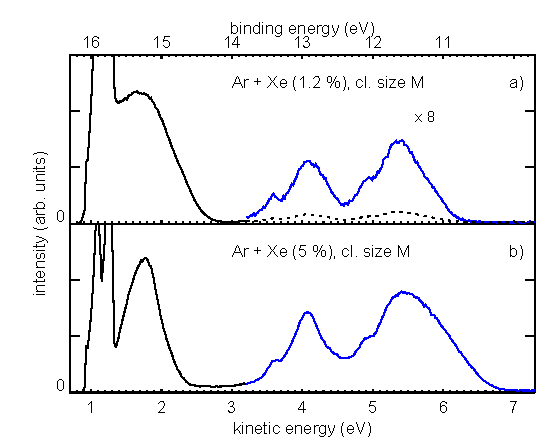
\includegraphics[width=8.5cm]{pics/figure_oval_2.pdf}
 \caption{
Outer valence spectra of mixed Ar-Xe clusters from gas mixtures with different Xe concentration. See Fig.\ \ref{figure:oval1} and text for details.
}
 \label{figure:oval2}
\end{figure}

